

\documentclass[english]{beamer}
\usepackage{mathptmx}
\usepackage[T1]{fontenc}
\usepackage[utf8]{luainputenc}
\usepackage{amsmath}
\usepackage{amssymb}
\usepackage{graphicx}

\makeatletter

%%%%%%%%%%%%%%%%%%%%%%%%%%%%%% LyX specific LaTeX commands.
%% A simple dot to overcome graphicx limitations
\newcommand{\lyxdot}{.}


%%%%%%%%%%%%%%%%%%%%%%%%%%%%%% Textclass specific LaTeX commands.
 % this default might be overridden by plain title style
 \newcommand\makebeamertitle{\frame{\maketitle}}%
 \AtBeginDocument{
   \let\origtableofcontents=\tableofcontents
   \def\tableofcontents{\@ifnextchar[{\origtableofcontents}{\gobbletableofcontents}}
   \def\gobbletableofcontents#1{\origtableofcontents}
 }
 \long\def\lyxframe#1{\@lyxframe#1\@lyxframestop}%
 \def\@lyxframe{\@ifnextchar<{\@@lyxframe}{\@@lyxframe<*>}}%
 \def\@@lyxframe<#1>{\@ifnextchar[{\@@@lyxframe<#1>}{\@@@lyxframe<#1>[]}}
 \def\@@@lyxframe<#1>[{\@ifnextchar<{\@@@@@lyxframe<#1>[}{\@@@@lyxframe<#1>[<*>][}}
 \def\@@@@@lyxframe<#1>[#2]{\@ifnextchar[{\@@@@lyxframe<#1>[#2]}{\@@@@lyxframe<#1>[#2][]}}
 \long\def\@@@@lyxframe<#1>[#2][#3]#4\@lyxframestop#5\lyxframeend{%
   \frame<#1>[#2][#3]{\frametitle{#4}#5}}
 \def\lyxframeend{} % In case there is a superfluous frame end

%%%%%%%%%%%%%%%%%%%%%%%%%%%%%% User specified LaTeX commands.
\usetheme{Warsaw}
%\usetheme{Boadilla}
% or ...


\usecolortheme{orchid}
\setbeamertemplate{footline}[text line]{} % makes the footer EMPTY

\setbeamercovered{transparent}
% or whatever (possibly just delete it)

\makeatother

\usepackage{babel}
\begin{document}

\title{Daily urban mobility using agent-based modeling}


\author{Bernadette, Christoph, Claire, Florent, Nicolas, Juste}


\date{CSSS2013 Group Project}

\makebeamertitle

\lyxframeend{}\section{Framework}


\lyxframeend{}\subsection{Context and problem}


\lyxframeend{}\lyxframe{Context and problem}
\begin{itemize}
\item General framework : problem of daily travels of individuals inside
a city.


\pause{}

\item Already a lot of literature (MIRO 2012, Mobisim 2013 , ...), complicated
models in huge projects.


\pause{}

\item Problematic : to obtain a simple model {[}F(S,S,C){]} to express multimodal
transport shares and local flows functions over a standard day.
\end{itemize}

\lyxframeend{}\subsection{Objectives and Methodology}


\lyxframeend{}\lyxframe{Objectives}
\begin{itemize}
\item Simple but rigourous model.


\pause{}

\item Integration of real data (GIS work) 


\pause{}

\item Apply the model on a test case (e. g. optimal implantation of a new
transportation infrastructure)
\end{itemize}

\lyxframeend{}\lyxframe{Methodology}

\begin{figure}
\hfill{}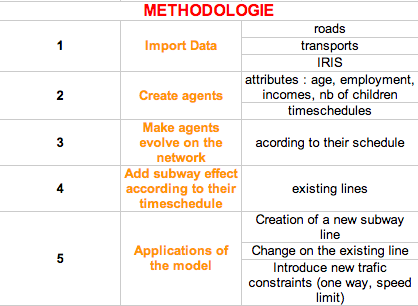
\includegraphics[scale=0.6]{methodoProject}\hfill{}\hfill{}\caption{Model conception methodology}
\end{figure}



\lyxframeend{}\section{Main identified issues}


\lyxframeend{}\subsection{Theoretical issues}


\lyxframeend{}\lyxframe{Theoretical issues}
\begin{itemize}
\item Urban social systems are highly heterogeneous.


\pause{}

\item Human decisions modeling.


\pause{}

\item Scaling.
\end{itemize}

\lyxframeend{}\subsection{Practical issues}


\lyxframeend{}\lyxframe{Practical issues}
\begin{itemize}
\item Group organisation: multi-disciplinary work


\pause{}

\item Time


\pause{}

\item Data collection and treatment
\end{itemize}

\lyxframeend{}\section{Achieved work and perspectives}


\lyxframeend{}\subsection{Achieved work}


\lyxframeend{}\lyxframe{Achieved work}
\begin{itemize}
\item Reframed the problem.


\pause{}

\item Collected the data.


\pause{}

\item Drafted a workplan
\end{itemize}

\lyxframeend{}\subsection{Perspectives}


\lyxframeend{}\lyxframe{Perspectives}
\begin{itemize}
\item Import data in NetLogo


\pause{}

\item Create agents


\pause{}

\item Make them interact between each other and with networks


\pause{}

\item Explore the model
\end{itemize}

\lyxframeend{}\lyxframe{Questions}

{\LARGE \hfill{}?\hfill{}\hfill{}}{\LARGE \par}

{\LARGE \hfill{}}\includegraphics[scale=0.25]{\string"/Users/Juste/Desktop/Capture d’écran 2013-07-12 à 18.01.33\string".png}{\LARGE \hfill{}\hfill{}}{\LARGE \par}


\lyxframeend{}
\end{document}
